\begin{frame}
  \frametitle{Fission Chain Reaction}
  % a comment
  \begin{figure}[htbp!]
    \begin{center}
      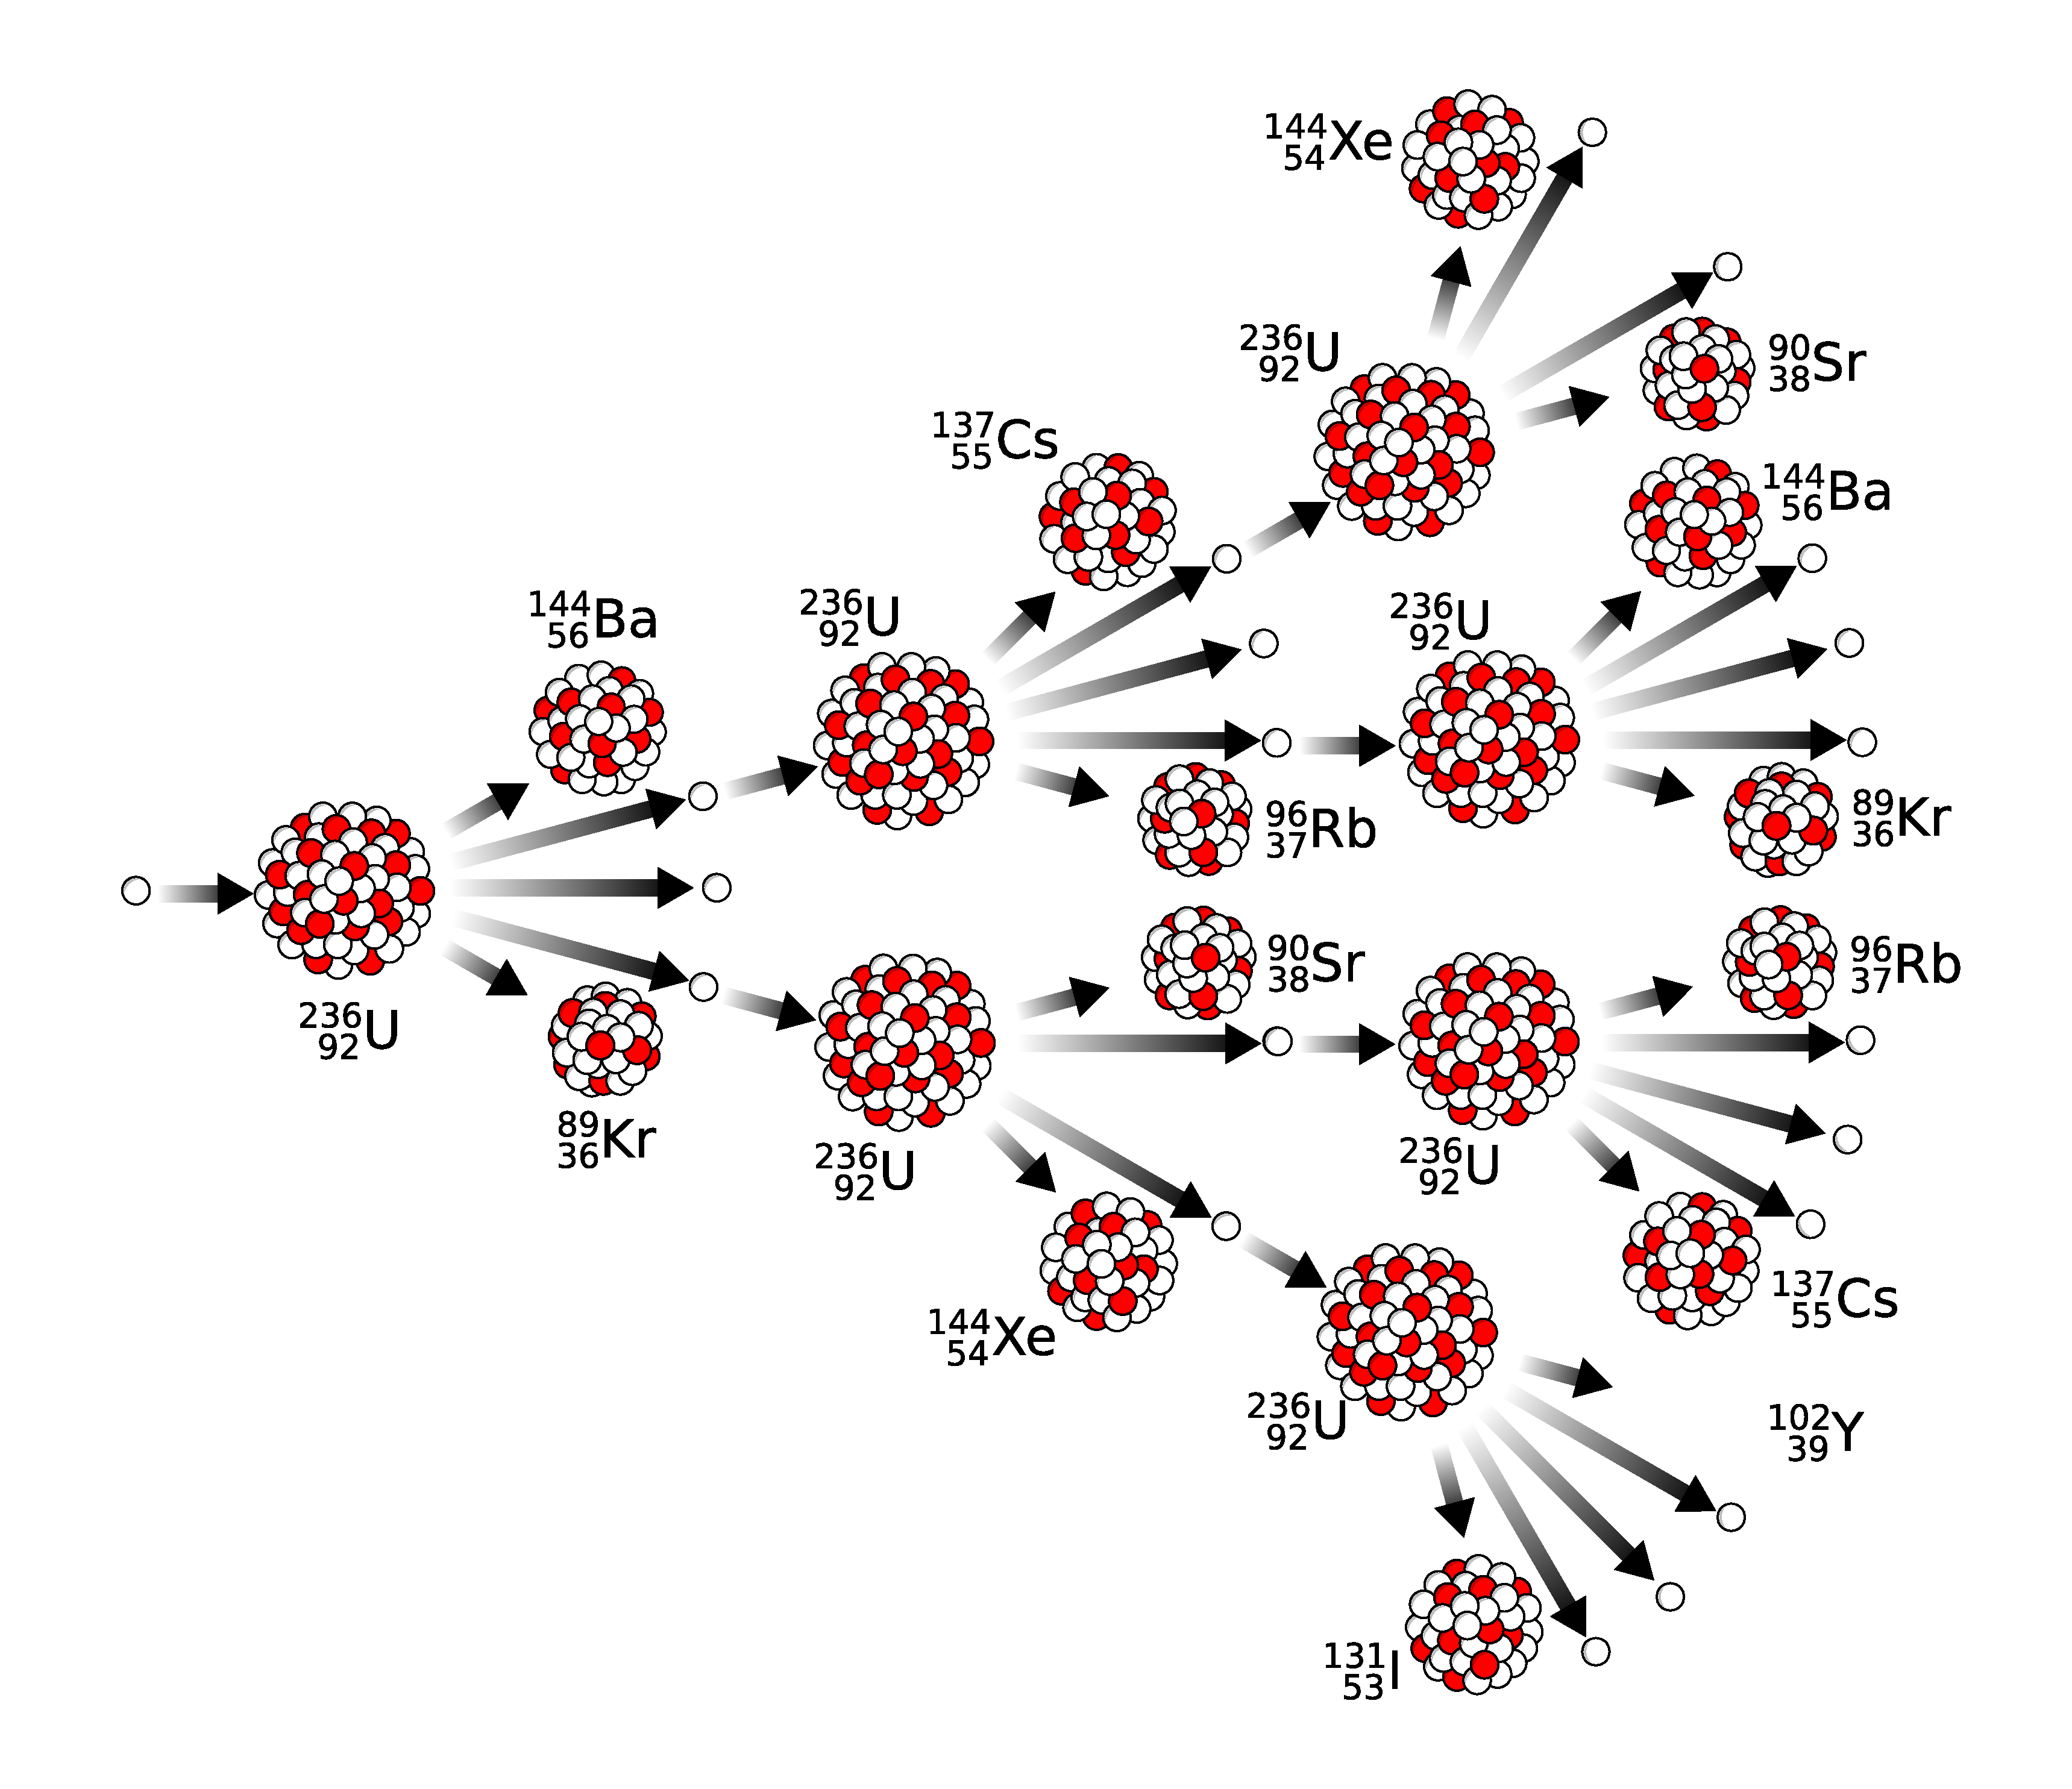
\includegraphics[height=6cm]{./images/Nuclear_fission_chain_reaction.pdf}
    \end{center}
          \caption{Diagram of a fission chain reaction, from
          \cite{nuclear_wikipedia_2017}.}
    \label{fig:fisson-reaction}
  \end{figure}
\end{frame}

\begin{frame}
    \frametitle{Depletion}
        \begin{columns}
            \column[t]{5cm}
                From Duderstadt \& Hamilton, Nuclear Reactor Analysis:
                \begin{quote}
                        The atomic densities of various isotopes in a reactor
                        core are continually changing due to niclear processes
                        such as fission, neutron capture, and radioactive decay
                \end{quote}
                

                Why do we care?
            \column[t]{5cm}
                \begin{figure}[htbp!]
                    \begin{center}
                        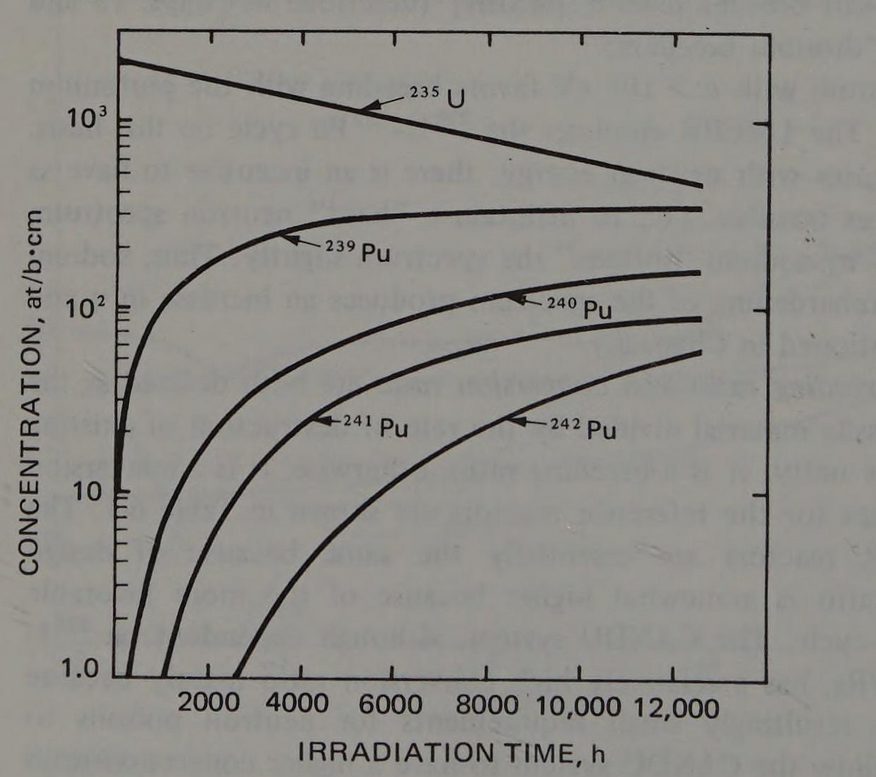
\includegraphics[height=5cm]{./images/isotopes_over_time.png}
                    \end{center}
                    \caption{Buildup of plutionium isotopes with a burnup for a
                    typical LWR fuel composition. Reproduced from Figure 6-2 in
                    \cite{knief_nuclear_1981}.}
                    \label{fig:isotopes-over-time}
                \end{figure}
        \end{columns}
\end{frame}

\begin{frame}
    \frametitle{Depletion makes everything {\it more} expensive}     
        \begin{columns}
            \column[t]{5cm}
               \begin{itemize}
                    \item Thousands of nuclides
                    \item Rections must be stored
                    \item Compositions must be stored
                \end{itemize}

                \begin{figure}[htbp]
                    \begin{center}
                        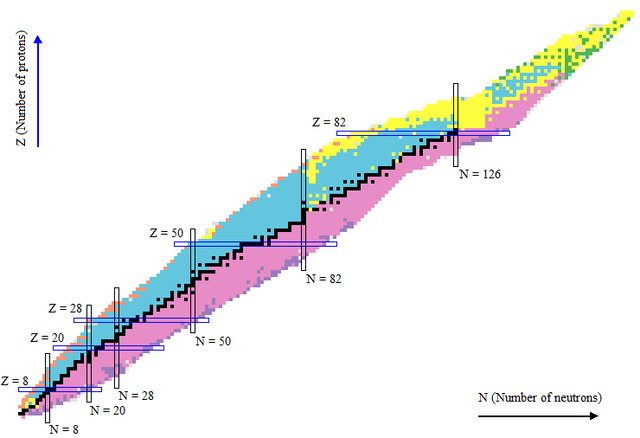
\includegraphics[height=3cm]{./images/nuclide_table.jpg}
                    \end{center}
                    \caption{Table of Nuclides. Z on y-axis, N on x-axis. From
                    \cite{tracy_jr_binding_2017}}
                    \label{fig:nuclide-table}
                \end{figure}
            \column[t]{5cm}
                \begin{figure}[htbp]
                    \begin{center}
                        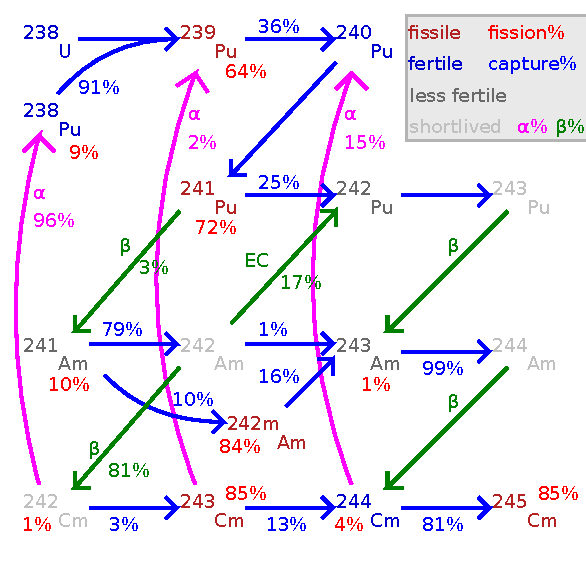
\includegraphics[height=5cm]{./images/pu-chain.pdf}
                    \end{center}
                    \caption{Example of the complicated web of production and
                    transmutation reactions. From \cite{wikipedia_magyar_2007}}
                    \label{fig:pu-chain}
                \end{figure}
        \end{columns}
\end{frame}


